\chapter{TESTING AND EVALUATION RESULTS}

\section{Usability Testing}

\textbf{Volunteer 1}
\begin{figure}[htb]
  \centering
  \subfloat[][Adobe Photoshop]{\label{fig:ResultPhotoshop1}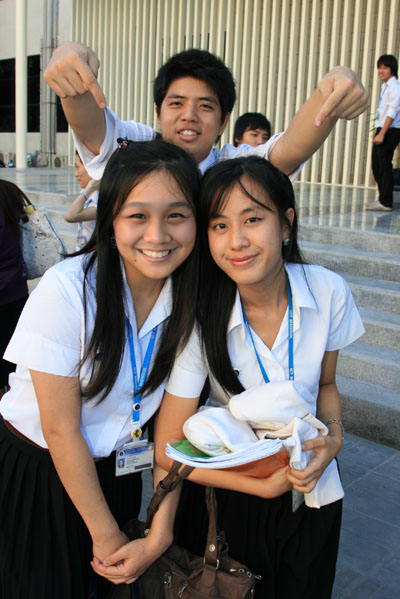
\includegraphics[width=0.3\textwidth]{photoshop1.png}}
  \subfloat[][Face Replacement]{\label{fig:ResultFaceReplacement1}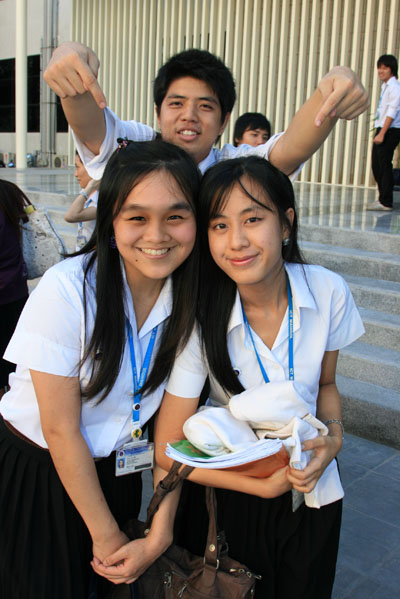
\includegraphics[width=0.3\textwidth]{facereplacement1.png}}
  \caption{The Output Images created by Volunteer 1}
  \label{fig:Result1}
\end{figure}

\begin{center}
\begin{tabular}{|c|c|c|}
  \hline
  % after \\: \hline or \cline{col1-col2} \cline{col3-col4} ...
  Method & The required time & The user satisfaction score \\ \hline
  Adobe Photoshop & 355 seconds & 70\% \\ \hline
  Face Replacement & 99 seconds & 60\% \\
  \hline
\end{tabular}
\end{center}

\vspace{0.2in}\noindent User interface comment from Volunteer 1

\emph{If possible, the program should have ability to adjust the offset, or to scale the contour.}

\vspace{2.0in}\noindent \textbf{Volunteer 2}
\begin{figure}[htb]
  \centering
  \subfloat[][Adobe Photoshop]{\label{fig:ResultPhotoshop2}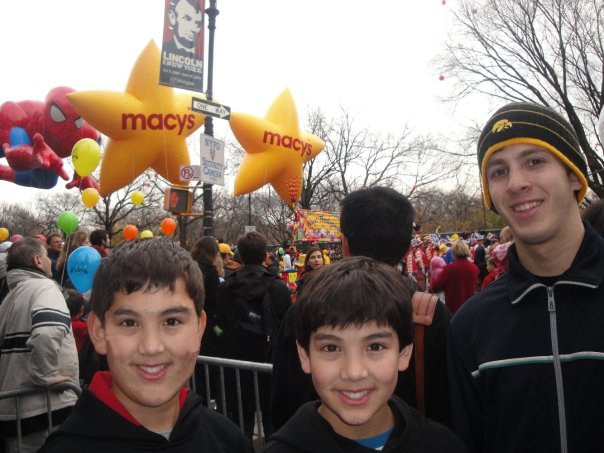
\includegraphics[width=0.3\textwidth]{photoshop2.png}}
  \subfloat[][Face Replacement]{\label{fig:ResultFaceReplacement2}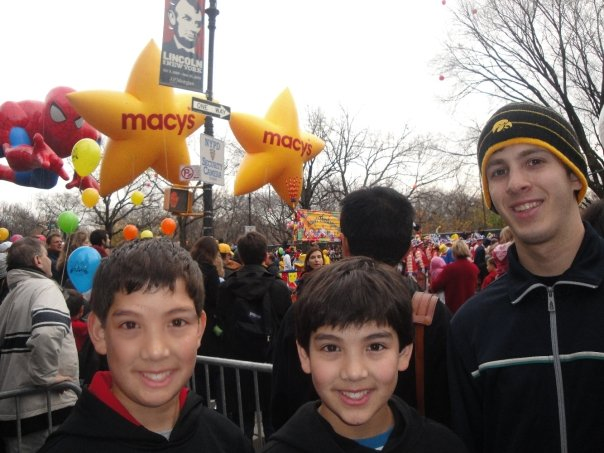
\includegraphics[width=0.3\textwidth]{facereplacement2.png}}
  \caption{The Output Images created by Volunteer 2}
  \label{fig:Result2}
\end{figure}

\begin{center}
\begin{tabular}{|c|c|c|}
  \hline
  % after \\: \hline or \cline{col1-col2} \cline{col3-col4} ...
  Method & The required time & The user satisfaction score \\ \hline
  Adobe Photoshop & 535 seconds & 40\% \\ \hline
  Face Replacement & 174 seconds & 65\% \\
  \hline
\end{tabular}
\end{center}

\vspace{0.2in}\noindent User interface comment from Volunteer 2

\emph{The objects behind the interface windows should not be seen. There should be a kind of Pop-Up to tell the instruction.}

\vspace{0.2in}\noindent \textbf{Volunteer 3}
\begin{figure}[htb]
  \centering
  \subfloat[][Adobe Photoshop]{\label{fig:ResultPhotoshop3}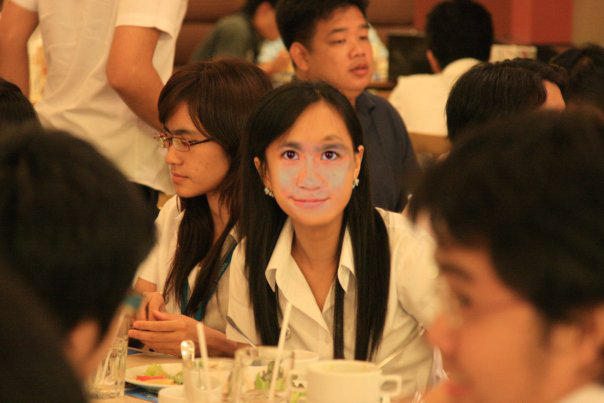
\includegraphics[width=0.3\textwidth]{photoshop3.png}}
  \subfloat[][Face Replacement]{\label{fig:ResultFaceReplacement3}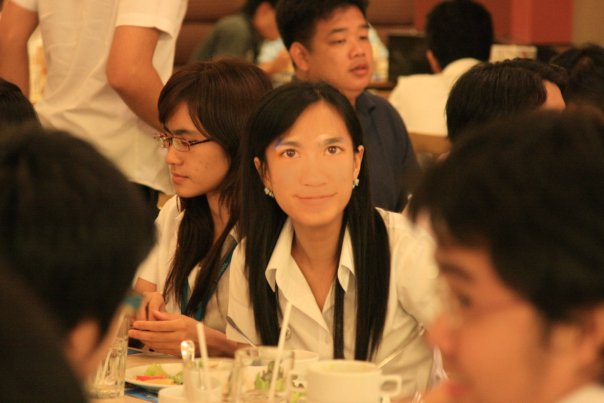
\includegraphics[width=0.3\textwidth]{facereplacement3.png}}
  \caption{The Output Images created by Volunteer 3}
  \label{fig:Result3}
\end{figure}

\vspace{1.0in}
\begin{center}
\begin{tabular}{|c|c|c|}
  \hline
  % after \\: \hline or \cline{col1-col2} \cline{col3-col4} ...
  Method & The required time & The user satisfaction score \\ \hline
  Adobe Photoshop & 1069 seconds & 40\% \\ \hline
  Face Replacement & 323 seconds & 60\% \\
  \hline
\end{tabular}
\end{center}

\vspace{0.2in}\noindent User interface comment from Volunteer 3

\emph{The icons behind the interface can be seen when run on a desktop.}

\vspace{0.2in}\noindent \textbf{Volunteer 4}
\begin{figure}[htb]
  \centering
  \subfloat[][Adobe Photoshop]{\label{fig:ResultPhotoshop4}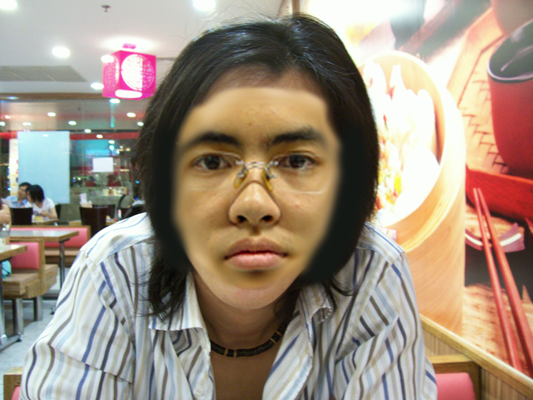
\includegraphics[width=0.3\textwidth]{photoshop4.png}}
  \subfloat[][Face Replacement]{\label{fig:ResultFaceReplacement4}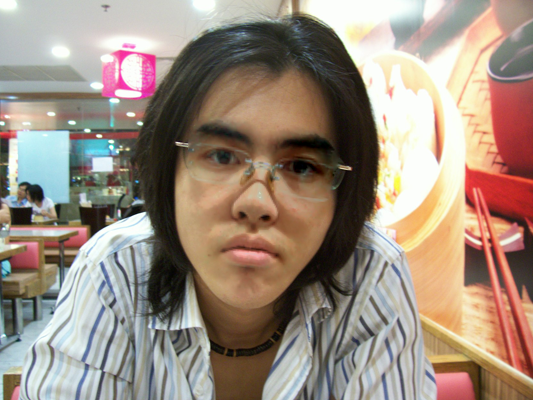
\includegraphics[width=0.3\textwidth]{facereplacement4.png}}
  \caption{The Output Images created by Volunteer 4}
  \label{fig:Result4}
\end{figure}

\begin{center}
\begin{tabular}{|c|c|c|}
  \hline
  % after \\: \hline or \cline{col1-col2} \cline{col3-col4} ...
  Method & The required time & The user satisfaction score \\ \hline
  Adobe Photoshop & 1016 seconds & 10\% \\ \hline
  Face Replacement & 293 seconds & 91\% \\
  \hline
\end{tabular}
\end{center}

\vspace{0.2in}\noindent User interface comment from Volunteer 4

\emph{There are no instructions to use the program. Other users who use it for the first time will have no idea how to use it.}

\vspace{2.5in}\noindent \textbf{Volunteer 5}
\begin{figure}[htb]
  \centering
  \subfloat[][Adobe Photoshop]{\label{fig:ResultPhotoshop5}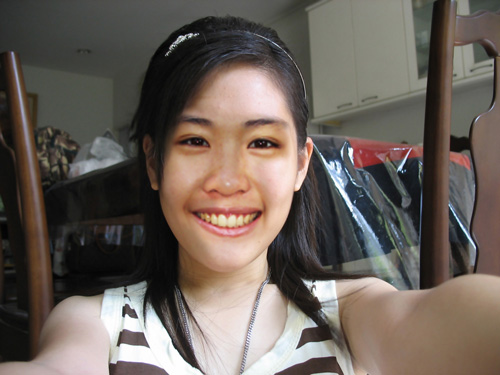
\includegraphics[width=0.3\textwidth]{photoshop5.png}}
  \subfloat[][Face Replacement]{\label{fig:ResultFaceReplacement5}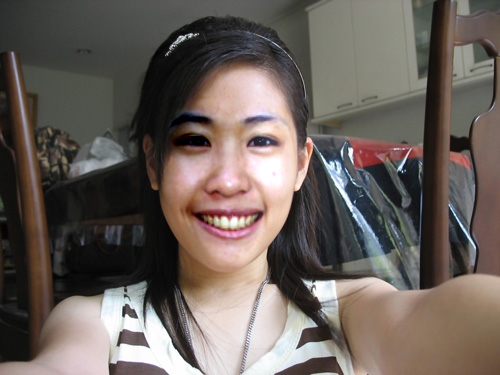
\includegraphics[width=0.3\textwidth]{facereplacement5.png}}
  \caption{The Output Images created by Volunteer 5}
  \label{fig:Result5}
\end{figure}

\begin{center}
\begin{tabular}{|c|c|c|}
  \hline
  % after \\: \hline or \cline{col1-col2} \cline{col3-col4} ...
  Method & The required time & The user satisfaction score \\ \hline
  Adobe Photoshop & 352 seconds & 45\% \\ \hline
  Face Replacement & 317 seconds & 85\% \\
  \hline
\end{tabular}
\end{center}

\vspace{0.2in}\noindent User interface comment from Volunteer 5

\emph{The Save button should be on the above panel. The image on the Edit button should also be changed. There should be a 'Getting Started' feature.}

\vspace{0.2in}\noindent \textbf{Volunteer 6}
\begin{figure}[htb]
  \centering
  \subfloat[][Adobe Photoshop]{\label{fig:ResultPhotoshop6}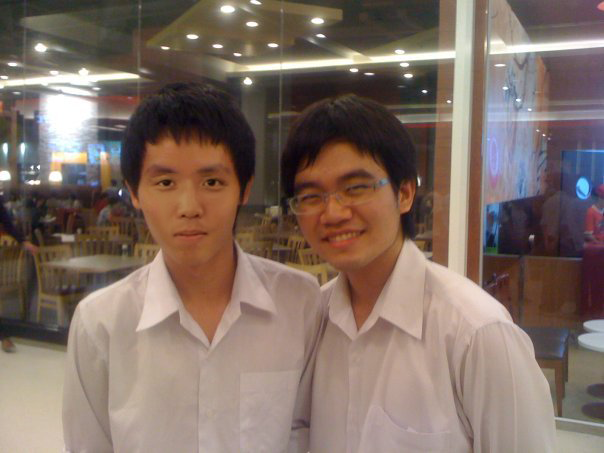
\includegraphics[width=0.3\textwidth]{photoshop6.png}}
  \subfloat[][Face Replacement]{\label{fig:ResultFaceReplacement6}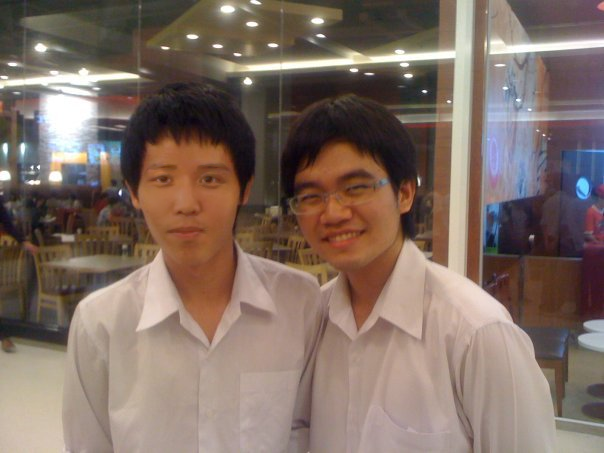
\includegraphics[width=0.3\textwidth]{facereplacement6.png}}
  \caption{The Output Images created by Volunteer 6}
  \label{fig:Result6}
\end{figure}

\vspace{1.0in}
\begin{center}
\begin{tabular}{|c|c|c|}
  \hline
  % after \\: \hline or \cline{col1-col2} \cline{col3-col4} ...
  Method & The required time & The user satisfaction score \\ \hline
  Adobe Photoshop & 575 seconds & 60\% \\ \hline
  Face Replacement & 287 seconds & 55\% \\
  \hline
\end{tabular}
\end{center}

\vspace{0.2in}\noindent User interface comment from Volunteer 6

\emph{Users may want to zoom the image to easily edit the contour. Users may have no idea how to use some features, such as users can double click on the face to revert the contour.}

\vspace{0.2in}\noindent \textbf{Volunteer 7}
\begin{figure}[htb]
  \centering
  \subfloat[][Adobe Photoshop]{\label{fig:ResultPhotoshop7}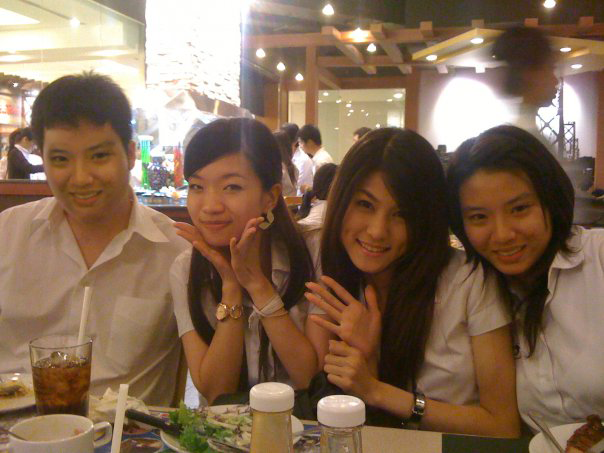
\includegraphics[width=0.3\textwidth]{photoshop7.png}}
  \subfloat[][Face Replacement]{\label{fig:ResultFaceReplacement7}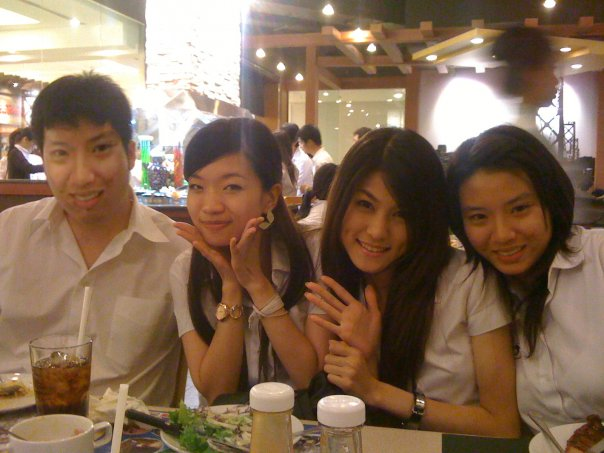
\includegraphics[width=0.3\textwidth]{facereplacement7.png}}
  \caption{The Output Images created by Volunteer 7}
  \label{fig:Result7}
\end{figure}

\begin{center}
\begin{tabular}{|c|c|c|}
  \hline
  % after \\: \hline or \cline{col1-col2} \cline{col3-col4} ...
  Method & The required time & The user satisfaction score \\ \hline
  Adobe Photoshop & 461 seconds & 65\% \\ \hline
  Face Replacement & 225 seconds & 65\% \\
  \hline
\end{tabular}
\end{center}

\vspace{0.2in}\noindent User interface comment from Volunteer 7

\emph{Some users may have no idea about the techniques they have to select in the option menu. To correctly edit the contour is a bit difficult to achieve.}

\begin{center}
\begin{tabular}{|c|c|c|c|} % centered columns (4 columns)
\hline
Volunteer & Adobe Photoshop & Face Replacement \\ % inserts table heading
\hline % inserts single horizontal line
1 & 355 & 99 \\ % inserting body of the table
2 & 535 & 174 \\
3 & 1069 & 323 \\
4 & 1016 & 293 \\
5 & 352 & 317 \\
6 & 575 & 287 \\
7 & 461 & 225 \\
\hline\hline
Average & 625.29 & 245.42 \\
\hline
\end{tabular}
\end{center}

\vspace{0.2in}The table above shows the required time results (in seconds) from all volunteers and the mean average required time from both methods. The table below shows the user satisfaction scores (in \%) from all volunteers and the mean average scores from both methods.
\vspace{0.2in}

\begin{center}
\begin{tabular}{|c|c|c|c|} % centered columns (4 columns)
\hline
Volunteer & Adobe Photoshop & Face Replacement \\ % inserts table heading
\hline % inserts single horizontal line
1 & 70\% & 60\% \\ % inserting body of the table
2 & 40\% & 65\% \\
3 & 40\% & 60\% \\
4 & 10\% & 91\% \\
5 & 45\% & 85\% \\
6 & 60\% & 55\% \\
7 & 65\% & 65\% \\
\hline\hline
Average & 47\% & 70\% \\
\hline
\end{tabular}
\end{center}

\section{Output Quality Evaluation}

\vspace{0.2in}
\begin{center}
\begin{tabular}{|c|c|c|c|c|c||c|}
\hline
\multicolumn{7}{|c|}{Volunteer} \\
% \hline
\cline{2-7}
Figure & 1 & 2 & 3 & 4 & 5 & Average\\
\hline
A.1 (a) & 100\% & 100\% & 97\% & 100\% & 100\% & 99.4\% \\
A.1 (b) & 70\% & 80\% & 15\% & 65\% & 90\% & 64\% \\
A.2 (a) & 50\% & 5\% & 5\% & 50\% & 30\% & 28\% \\
A.2 (b) & 100\% & 70\% & 65\% & 40\% & 70\% & 69\% \\
A.3 (a) & 0\% & 10\% & 10\% & 0\% & 25\% & 9\% \\
A.3 (b) & 30\% & 10\% & 5\% & 0\% & 30\% & 15\% \\
A.4 (a) & 0\% & 20\% & 25\% & 0\% & 30\% & 15\% \\
A.4 (b) & 100\% & 90\% & 45\% & 55\% & 40\% & 66\% \\
A.5 (a) & 80\% & 70\% & 95\% & 65\% & 80\% & 78\% \\
A.5 (b) & 50\% & 80\% & 85\% & 60\% & 90\% & 73\% \\
A.6 (a) & 80\% & 65\% & 67\% & 100\% & 70\% & 76.4\% \\
A.6 (b) & 90\% & 60\% & 30\% & 60\% & 70\% & 62\% \\
A.7 (a) & 95\% & 75\% & 55\% & 50\% & 70\% & 69\% \\
A.7 (b) & 20\% & 20\% & 5\% & 0\% & 30\% & 15\% \\
\hline
\end{tabular}
\end{center}

\vspace{0.2in}The table above shows the results of output quality satisfaction scores and the mean average score of each output image. From these results, the mean average quality scores for both methods are shown in the table below.
\vspace{0.2in}

\begin{center}
\begin{tabular}{|c|c|}
  \hline
  Method & Average quality score \\ \hline
  Adobe Photoshop & 53\% \\
  Face Replacement & 52\% \\
  \hline
\end{tabular}
\end{center} 